\chapter{有向图}
  \begin{Def}
    设$V$为一个有穷非空集合,$A \subseteq V\times V \setminus \{(v,v)|v \in V\}$,二元组$D=(V,A)$称为一个{\bfseries 有向图}。$V$称为有向图$D$的{\bfseries 顶点集},$V$中的元素称为$D$的{\bfseries 顶点}。
    $A$称为$D$的{\bfseries 弧集}或{\bfseries 有向边集},$A$中的元素称为$D$的{\bfseries 弧}或{\bfseries 有向边}。如果$x = (u,v) \in A$,则$u$称为弧$x$的{\bfseries 起点},$v$称为弧$x$的{\bfseries 终点}。
  \end{Def}
    \centering
  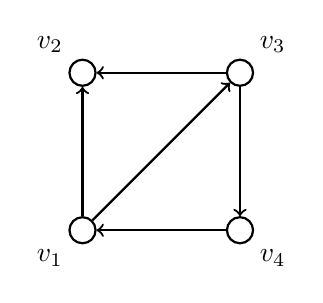
\begin{tikzpicture}[auto,
    specification/.style ={circle, draw, thick}]
   \node[specification] (A) [label=-135:$v_1$] at (0,0)  {};
   \node[specification] (B) [label=135:$v_2$] at (0,2)  {};
   \node[specification] (C) [label=45:$v_3$] at (2,2)  {};
   \node[specification] (D) [label=-45:$v_4$] at (2,0)  {};
   \draw[thick, ->] (A) to  (B);
   \draw[thick, ->] (C) to  (B);
   \draw[thick, ->] (C) to  (D);
   \draw[thick, ->] (D) to  (A);
   \draw[thick, ->] (A) to  (C);
\end{tikzpicture}

  \begin{Def}
    如果$(u,v)$和$(v,u)$都是有向图$D$的弧,则称$(u,v)$与$(v,u)$为$D$的{\bfseries 对
      称弧}。如果$D$中不含对称弧,则称$D$为{\bfseries 定向图}。
  \end{Def}
  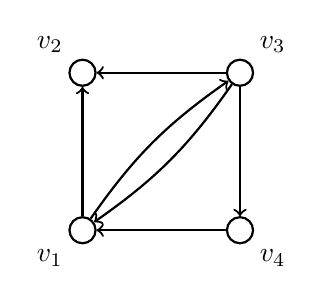
\begin{tikzpicture}[auto,
    specification/.style ={circle, draw, thick}]
   \node[specification] (A) [label=-135:$v_1$] at (0,0)  {};
   \node[specification] (B) [label=135:$v_2$] at (0,2)  {};
   \node[specification] (C) [label=45:$v_3$] at (2,2)  {};
   \node[specification] (D) [label=-45:$v_4$] at (2,0)  {};
   \draw[thick, ->] (A) to  (B);
   \draw[thick, ->] (C) to  (B);
   \draw[thick, ->] (C) to  (D);
   \draw[thick, ->] (D) to  (A);
   \draw[thick, ->] (A) to [bend left = 10] (C);
   \draw[thick, ->] (C) to [bend left = 10] (A);
\end{tikzpicture}\hspace{1cm}
  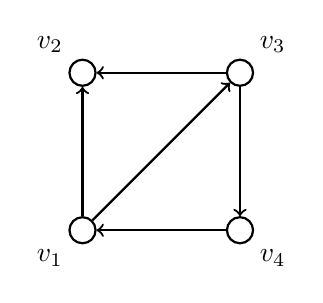
\begin{tikzpicture}[auto,
    specification/.style ={circle, draw, thick}]
   \node[specification] (A) [label=-135:$v_1$] at (0,0)  {};
   \node[specification] (B) [label=135:$v_2$] at (0,2)  {};
   \node[specification] (C) [label=45:$v_3$] at (2,2)  {};
   \node[specification] (D) [label=-45:$v_4$] at (2,0)  {};
   \draw[thick, ->] (A) to  (B);
   \draw[thick, ->] (C) to  (B);
   \draw[thick, ->] (C) to  (D);
   \draw[thick, ->] (D) to  (A);
   \draw[thick, ->] (A) to  (C);
\end{tikzpicture}

  \begin{Def}
    设$D=(V,A)$为一个有向图,$D$的{\bfseries 反向图}为有向图$D^T=(V,A^T)$,其中
    \[A^T=\{(u,v)|(v,u)\in A\}\]
  \end{Def}
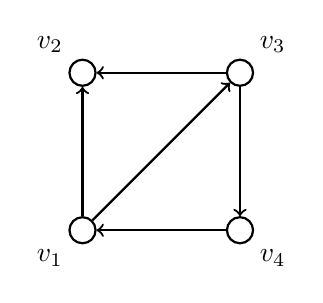
\begin{tikzpicture}[auto,
    specification/.style ={circle, draw, thick}]
   \node[specification] (A) [label=-135:$v_1$] at (0,0)  {};
   \node[specification] (B) [label=135:$v_2$] at (0,2)  {};
   \node[specification] (C) [label=45:$v_3$] at (2,2)  {};
   \node[specification] (D) [label=-45:$v_4$] at (2,0)  {};
   \draw[thick, ->] (A) to  (B);
   \draw[thick, ->] (C) to  (B);
   \draw[thick, ->] (C) to  (D);
   \draw[thick, ->] (D) to  (A);
   \draw[thick, ->] (A) to  (C);
\end{tikzpicture}\hspace{1cm}
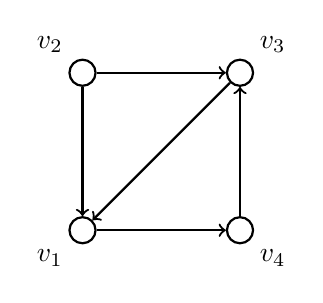
\begin{tikzpicture}[auto,
    specification/.style ={circle, draw, thick}]
   \node[specification] (A) [label=-135:$v_1$] at (0,0)  {};
   \node[specification] (B) [label=135:$v_2$] at (0,2)  {};
   \node[specification] (C) [label=45:$v_3$] at (2,2)  {};
   \node[specification] (D) [label=-45:$v_4$] at (2,0)  {};
   \draw[thick, ->] (B) to  (A);
   \draw[thick, ->] (B) to  (C);
   \draw[thick, ->] (D) to  (C);
   \draw[thick, ->] (A) to  (D);
   \draw[thick, ->] (C) to  (A);
\end{tikzpicture}

  \begin{Def}
    设$D=(V,A)$为一个有向图,$v$为$D$的任一顶点,以$v$为终点的弧称为$v$的{\bfseries 入弧};以$v$为始点的弧称为$v$的{\bfseries 出弧}。顶点$v$的入弧的条数称为$v$的{\bfseries 入度},记为$id(v)$;顶点$v$的出弧的条数称为$v$的{\bfseries 出度},记为$od(v)$。
  \end{Def}
\centering
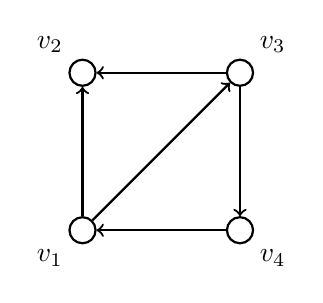
\begin{tikzpicture}[auto,
    specification/.style ={circle, draw, thick}]
   \node[specification] (A) [label=-135:$v_1$] at (0,0)  {};
   \node[specification] (B) [label=135:$v_2$] at (0,2)  {};
   \node[specification] (C) [label=45:$v_3$] at (2,2)  {};
   \node[specification] (D) [label=-45:$v_4$] at (2,0)  {};
   \draw[thick, ->] (A) to  (B);
   \draw[thick, ->] (C) to  (B);
   \draw[thick, ->] (C) to  (D);
   \draw[thick, ->] (D) to  (A);
   \draw[thick, ->] (A) to  (C);
 \end{tikzpicture}
     \begin{Thm}
      设$D=(V,A)$为一个有向图,$|A| = q$,则
      \[\sum_{v\in V}id(v) = \sum_{v\in V}od(v) = q\]
      从而
      \[\sum_{v\in V}(id(v) + od(v)) = 2q\]
  \end{Thm}
\centering
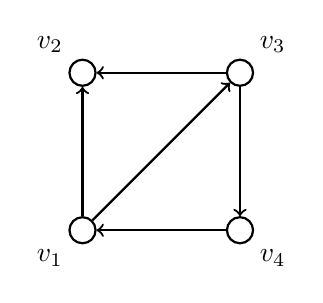
\begin{tikzpicture}[auto,
    specification/.style ={circle, draw, thick}]
   \node[specification] (A) [label=-135:$v_1$] at (0,0)  {};
   \node[specification] (B) [label=135:$v_2$] at (0,2)  {};
   \node[specification] (C) [label=45:$v_3$] at (2,2)  {};
   \node[specification] (D) [label=-45:$v_4$] at (2,0)  {};
   \draw[thick, ->] (A) to  (B);
   \draw[thick, ->] (C) to  (B);
   \draw[thick, ->] (C) to  (D);
   \draw[thick, ->] (D) to  (A);
   \draw[thick, ->] (A) to  (C);
\end{tikzpicture}  

  \begin{Def}
     有向图$D=(V,A)$称为{\bfseries 完全有向图},如果\[A=V\times V \setminus \{(v,v)| v \in V\}\]
   \end{Def}
   \centering
  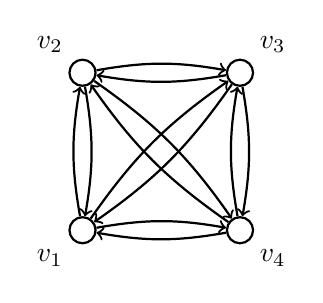
\begin{tikzpicture}[auto,
    specification/.style ={circle, draw, thick}]
   \node[specification] (A) [label=-135:$v_1$] at (0,0)  {};
   \node[specification] (B) [label=135:$v_2$] at (0,2)  {};
   \node[specification] (C) [label=45:$v_3$] at (2,2)  {};
   \node[specification] (D) [label=-45:$v_4$] at (2,0)  {};
   \draw[thick, ->] (A) to [bend left = 10]  (B);
   \draw[thick, ->] (B) to [bend left = 10]  (A);
   \draw[thick, ->] (B) to [bend left = 10]  (C);
   \draw[thick, ->] (C) to [bend left = 10]  (B);
   \draw[thick, ->] (C) to [bend left = 10]  (D);
   \draw[thick, ->] (D) to [bend left = 10]  (C);
   \draw[thick, ->] (D) to [bend left = 10]  (A);
   \draw[thick, ->] (A) to [bend left = 10]  (D);
   \draw[thick, ->] (B) to [bend left = 10]  (D);
   \draw[thick, ->] (D) to [bend left = 10]  (B);
   \draw[thick, ->] (A) to [bend left = 10]  (C);
   \draw[thick, ->] (C) to [bend left = 10]  (A);
\end{tikzpicture}   

  \begin{Def}
    有向图$D=(V,A)$的{\bfseries 补图}定义为$D^c=(V,A^c)$,其中
    \[A^c=(V \times V \setminus \{(v,v)|v \in V\})\setminus A\]
  \end{Def}
  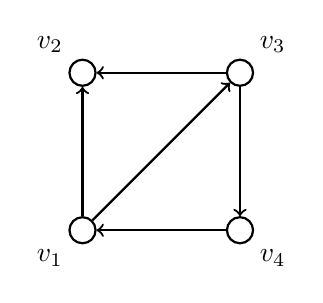
\begin{tikzpicture}[auto,
    specification/.style ={circle, draw, thick}]
   \node[specification] (A) [label=-135:$v_1$] at (0,0)  {};
   \node[specification] (B) [label=135:$v_2$] at (0,2)  {};
   \node[specification] (C) [label=45:$v_3$] at (2,2)  {};
   \node[specification] (D) [label=-45:$v_4$] at (2,0)  {};
   \draw[thick, ->] (A) to  (B);
   \draw[thick, ->] (C) to  (B);
   \draw[thick, ->] (C) to  (D);
   \draw[thick, ->] (D) to  (A);
   \draw[thick, ->] (A) to  (C);
 \end{tikzpicture}
\hspace{1cm}
 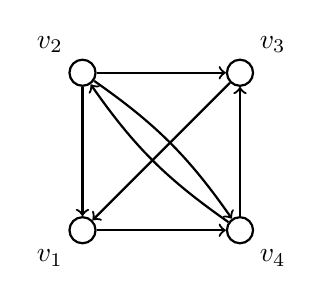
\begin{tikzpicture}[auto,
    specification/.style ={circle, draw, thick}]
   \node[specification] (A) [label=-135:$v_1$] at (0,0)  {};
   \node[specification] (B) [label=135:$v_2$] at (0,2)  {};
   \node[specification] (C) [label=45:$v_3$] at (2,2)  {};
   \node[specification] (D) [label=-45:$v_4$] at (2,0)  {};
   \draw[thick, ->] (B) to  (A);
   \draw[thick, ->] (B) to  (C);
   \draw[thick, ->] (D) to  (C);
   \draw[thick, ->] (A) to  (D);
   \draw[thick, ->] (C) to  (A);
   \draw[thick, ->] (B) to [bend left = 10]  (D);
   \draw[thick, ->] (D) to [bend left = 10]  (B);
\end{tikzpicture}

  \begin{Def}
    设$D_1=(V_1,A_1)$,$D_2=(V_2,A_2)$都为有向图,如果存在一个一一对应$\varphi:V_1 \to V_2$,使得$\forall u,v \in V_1, (u,v) \in A_1$当且仅当$(\varphi(u), \varphi(v)) \in A_2$,则称$D_1$与$D_2${\bfseries 同构}。
  \end{Def}
  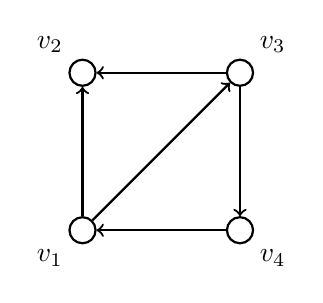
\begin{tikzpicture}[auto,
    specification/.style ={circle, draw, thick}]
   \node[specification] (A) [label=-135:$v_1$] at (0,0)  {};
   \node[specification] (B) [label=135:$v_2$] at (0,2)  {};
   \node[specification] (C) [label=45:$v_3$] at (2,2)  {};
   \node[specification] (D) [label=-45:$v_4$] at (2,0)  {};
   \draw[thick, ->] (A) to  (B);
   \draw[thick, ->] (C) to  (B);
   \draw[thick, ->] (C) to  (D);
   \draw[thick, ->] (D) to  (A);
   \draw[thick, ->] (A) to  (C);
 \end{tikzpicture}  \hspace{1cm}
   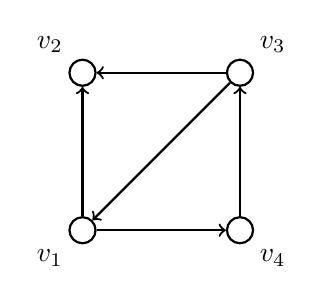
\begin{tikzpicture}[auto,
    specification/.style ={circle, draw, thick}]
   \node[specification] (A) [label=-135:$v_1$] at (0,0)  {};
   \node[specification] (B) [label=135:$v_2$] at (0,2)  {};
   \node[specification] (C) [label=45:$v_3$] at (2,2)  {};
   \node[specification] (D) [label=-45:$v_4$] at (2,0)  {};
   \draw[thick, ->] (A) to  (B);
   \draw[thick, ->] (C) to  (B);
   \draw[thick, ->] (D) to  (C);
   \draw[thick, ->] (C) to  (A);
   \draw[thick, ->] (A) to  (D);
\end{tikzpicture} 

  \begin{Def}
    设$D=(V,A)$为一个有向图。$D$的一条{\bfseries 有向通道}为$D$的顶点和弧的一个交错序列
    \[v_0,x_1,v_1,x_2,v_2,\cdots,v_{n-1},x_n,v_n \]
    其中$x_i = (v_{i-1},v_i)$, $i=1,2,\cdots, n$。$n$称为该有向通道的长。 这样的有向通道常称为$v_0-v_n$有向通道,并简记为$v_0v_1v_2\ldots v_n$。如果有向通道的长大于等于$1$且$v_0=v_n$,则称此有向通道为{\bfseries 闭有向通道}。
  \end{Def}
  \centering
  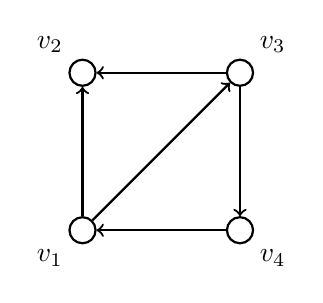
\begin{tikzpicture}[auto,
    specification/.style ={circle, draw, thick}]
   \node[specification] (A) [label=-135:$v_1$] at (0,0)  {};
   \node[specification] (B) [label=135:$v_2$] at (0,2)  {};
   \node[specification] (C) [label=45:$v_3$] at (2,2)  {};
   \node[specification] (D) [label=-45:$v_4$] at (2,0)  {};
   \draw[thick, ->] (A) to  (B);
   \draw[thick, ->] (C) to  (B);
   \draw[thick, ->] (C) to  (D);
   \draw[thick, ->] (D) to  (A);
   \draw[thick, ->] (A) to  (C);
 \end{tikzpicture}      
  \begin{Def}
如果有向图中一条有向通道的各弧互不相同,则称此有向通道为有向图的{\bfseries 有向迹}。如果一条闭有向通道上的各弧互不相同,则称此闭有向通道为{\bfseries 闭有向迹}。   
  \end{Def}
  \centering
  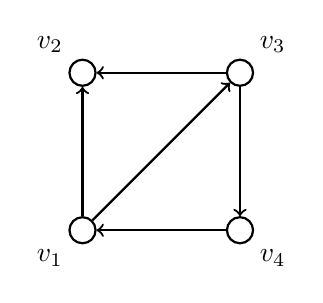
\begin{tikzpicture}[auto,
    specification/.style ={circle, draw, thick}]
   \node[specification] (A) [label=-135:$v_1$] at (0,0)  {};
   \node[specification] (B) [label=135:$v_2$] at (0,2)  {};
   \node[specification] (C) [label=45:$v_3$] at (2,2)  {};
   \node[specification] (D) [label=-45:$v_4$] at (2,0)  {};
   \draw[thick, ->] (A) to  (B);
   \draw[thick, ->] (C) to  (B);
   \draw[thick, ->] (C) to  (D);
   \draw[thick, ->] (D) to  (A);
   \draw[thick, ->] (A) to  (C);
 \end{tikzpicture}      
  \begin{Def}
如果一条有向迹上的各顶点互不相同,则称此有向迹为{\bfseries 有向路}。如果闭有向迹上除终点外各顶点互不相同,则称此闭有向迹为{\bfseries 有向圈},或{\bfseries 有向回路}。
  \end{Def}
  \centering
  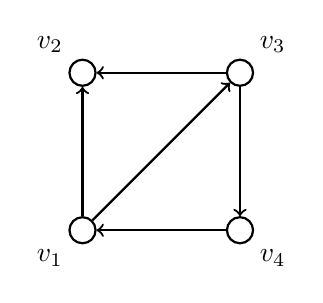
\begin{tikzpicture}[auto,
    specification/.style ={circle, draw, thick}]
   \node[specification] (A) [label=-135:$v_1$] at (0,0)  {};
   \node[specification] (B) [label=135:$v_2$] at (0,2)  {};
   \node[specification] (C) [label=45:$v_3$] at (2,2)  {};
   \node[specification] (D) [label=-45:$v_4$] at (2,0)  {};
   \draw[thick, ->] (A) to  (B);
   \draw[thick, ->] (C) to  (B);
   \draw[thick, ->] (C) to  (D);
   \draw[thick, ->] (D) to  (A);
   \draw[thick, ->] (A) to  (C);
 \end{tikzpicture}      

   \begin{Def}
含有向图$D$的所有顶点的有向圈称为$D$的{\bfseries 生成有向圈},或{\bfseries 有向哈密顿圈}。
有生成有向圈的有向图称为{\bfseries 有向哈密顿图}。含有向图$D$的所有顶点的有向路称为$D$的{\bfseries 生成有向路},
或{\bfseries 有向哈密顿路}。
  \end{Def}
  \centering
  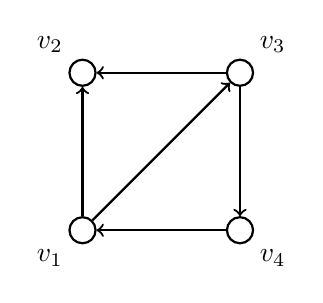
\begin{tikzpicture}[auto,
    specification/.style ={circle, draw, thick}]
   \node[specification] (A) [label=-135:$v_1$] at (0,0)  {};
   \node[specification] (B) [label=135:$v_2$] at (0,2)  {};
   \node[specification] (C) [label=45:$v_3$] at (2,2)  {};
   \node[specification] (D) [label=-45:$v_4$] at (2,0)  {};
   \draw[thick, ->] (A) to  (B);
   \draw[thick, ->] (C) to  (B);
   \draw[thick, ->] (C) to  (D);
   \draw[thick, ->] (D) to  (A);
   \draw[thick, ->] (A) to  (C);
 \end{tikzpicture}      

   \begin{Def}
    设$D=(V,A)$为一个有向图,$u$和$v$为$D$的顶点。如果在$D$中有一条从$u$到$v$的
    有向路,则称从$u$能达到$v$,或者$v$是从$u${\bfseries 可达}的。
  \end{Def}
  \centering
  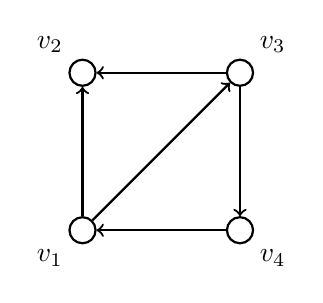
\begin{tikzpicture}[auto,
    specification/.style ={circle, draw, thick}]
   \node[specification] (A) [label=-135:$v_1$] at (0,0)  {};
   \node[specification] (B) [label=135:$v_2$] at (0,2)  {};
   \node[specification] (C) [label=45:$v_3$] at (2,2)  {};
   \node[specification] (D) [label=-45:$v_4$] at (2,0)  {};
   \draw[thick, ->] (A) to  (B);
   \draw[thick, ->] (C) to  (B);
   \draw[thick, ->] (C) to  (D);
   \draw[thick, ->] (D) to  (A);
   \draw[thick, ->] (A) to  (C);
 \end{tikzpicture}      


  \begin{Def}
   有向图$D$称为是{\bfseries 强连通}的,如果对$D$的任意两个不同的顶点$u$和$v$,$u$和$v$是互达的(即从$u$可以达到$v$并且从$v$可以达到$u$)。 
  \end{Def}
  \centering
  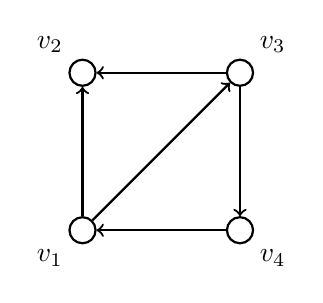
\begin{tikzpicture}[auto,
    specification/.style ={circle, draw, thick}]
   \node[specification] (A) [label=-135:$v_1$] at (0,0)  {};
   \node[specification] (B) [label=135:$v_2$] at (0,2)  {};
   \node[specification] (C) [label=45:$v_3$] at (2,2)  {};
   \node[specification] (D) [label=-45:$v_4$] at (2,0)  {};
   \draw[thick, ->] (A) to  (B);
   \draw[thick, ->] (C) to  (B);
   \draw[thick, ->] (C) to  (D);
   \draw[thick, ->] (D) to  (A);
   \draw[thick, ->] (A) to  (C);
 \end{tikzpicture}      

   \begin{Def}
   有向图$D$的极大强连通子图称为$D$的一个{\bfseries 强支}。 
  \end{Def}
  \centering
  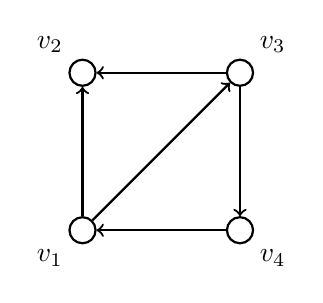
\begin{tikzpicture}[auto,
    specification/.style ={circle, draw, thick}]
   \node[specification] (A) [label=-135:$v_1$] at (0,0)  {};
   \node[specification] (B) [label=135:$v_2$] at (0,2)  {};
   \node[specification] (C) [label=45:$v_3$] at (2,2)  {};
   \node[specification] (D) [label=-45:$v_4$] at (2,0)  {};
   \draw[thick, ->] (A) to  (B);
   \draw[thick, ->] (C) to  (B);
   \draw[thick, ->] (C) to  (D);
   \draw[thick, ->] (D) to  (A);
   \draw[thick, ->] (A) to  (C);
 \end{tikzpicture}      

     \begin{Thm}
      设$D=(V,A)$为一个有向图。在$V$上定义二元关系$\cong$如下:\[\forall u, v \in V, u \cong v\text{当且仅当}u\text{与}v\text{互达}\]则$\cong$为$V$上的等价关系,$D$的强支就是关于$\cong$的每个等价类的导出子图。
  \end{Thm}
  \centering
  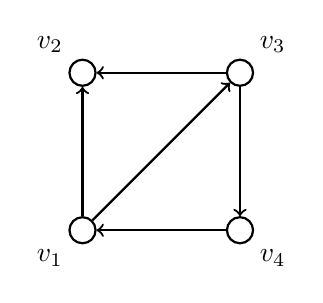
\begin{tikzpicture}[auto,
    specification/.style ={circle, draw, thick}]
   \node[specification] (A) [label=-135:$v_1$] at (0,0)  {};
   \node[specification] (B) [label=135:$v_2$] at (0,2)  {};
   \node[specification] (C) [label=45:$v_3$] at (2,2)  {};
   \node[specification] (D) [label=-45:$v_4$] at (2,0)  {};
   \draw[thick, ->] (A) to  (B);
   \draw[thick, ->] (C) to  (B);
   \draw[thick, ->] (C) to  (D);
   \draw[thick, ->] (D) to  (A);
   \draw[thick, ->] (A) to  (C);
 \end{tikzpicture}      

   \begin{Def}
   有向图$D=(V,A)$称为{\bfseries 单向连通}的,如果对$D$的任意两个不同的顶点$u$和$v$,或从$u$可达到$v$,或从$v$可达到$u$。 
  \end{Def}
  \centering
  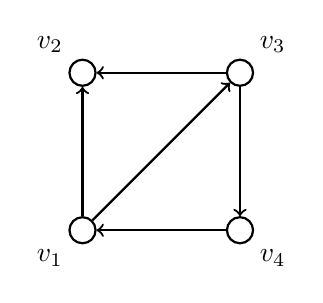
\begin{tikzpicture}[auto,
    specification/.style ={circle, draw, thick}]
   \node[specification] (A) [label=-135:$v_1$] at (0,0)  {};
   \node[specification] (B) [label=135:$v_2$] at (0,2)  {};
   \node[specification] (C) [label=45:$v_3$] at (2,2)  {};
   \node[specification] (D) [label=-45:$v_4$] at (2,0)  {};
   \draw[thick, ->] (A) to  (B);
   \draw[thick, ->] (C) to  (B);
   \draw[thick, ->] (C) to  (D);
   \draw[thick, ->] (D) to  (A);
   \draw[thick, ->] (A) to  (C);
 \end{tikzpicture}      

   \begin{Def}
   设$D=(V,A)$为一个有向图,如果抹去$D$中所有弧的方向之后所得到的无向图是连通的,则称$D$为{\bfseries 弱连通}的,简称{\bfseries 连通}的。 
  \end{Def}
  \centering
  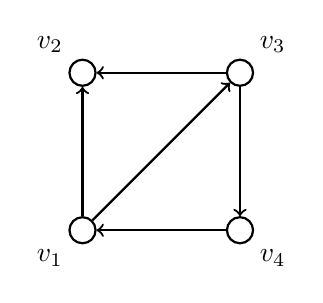
\begin{tikzpicture}[auto,
    specification/.style ={circle, draw, thick}]
   \node[specification] (A) [label=-135:$v_1$] at (0,0)  {};
   \node[specification] (B) [label=135:$v_2$] at (0,2)  {};
   \node[specification] (C) [label=45:$v_3$] at (2,2)  {};
   \node[specification] (D) [label=-45:$v_4$] at (2,0)  {};
   \draw[thick, ->] (A) to  (B);
   \draw[thick, ->] (C) to  (B);
   \draw[thick, ->] (C) to  (D);
   \draw[thick, ->] (D) to  (A);
   \draw[thick, ->] (A) to  (C);
 \end{tikzpicture}      

 \begin{Def}
   设$D=(V,A)$为一个有向图,$V=\{v_1,v_2,\ldots, v_p\}$,$p\times p$矩阵$B=(b_{ij})$称为$D$的邻接矩阵,其中
  \[b_{ij}=\begin{cases}
      1, \text{如果}(v_i,v_j)\in A\\
      0, \text{如果}(v_i,v_j)\notin A\\
    \end{cases}
  \]
 \end{Def}
   \begin{Thm}
   设$B$为有向图$D=(V,A)$的邻接矩阵,$V=\{v_1,v_2,\cdots,v_p\}$,则从顶点$v_i$到顶点$v_j$的长为$l$的有向通道的条数等于$B^l$的第$i$行第$j$列元素$(B^l)_{ij}$的值。 
  \end{Thm}
 \begin{Def}
   设$D=(V,A)$为一个有向图,$V=\{v_1,v_2,\ldots, v_p\}$,$p\times p$矩阵$R=(r_{ij})$称为$D$的可达矩阵,其中
  \[r_{ij}=\begin{cases}
      1, \text{如果从}v_i\text{可以达到}v_j\\
      0, \text{如果从}v_i\text{不能达到}v_j\\
    \end{cases}
  \]
 \end{Def}

    \begin{Thm}
    设$p \times p$矩阵$B$是有向图$D=(V,A)$的邻接矩阵,则$D$的可达矩阵
    \[R = I \lor B \lor B^{(2)} \lor \cdots \lor B^{(p-1)}\]
  \end{Thm}
  \begin{Thm}
   设$p \times p$矩阵$R$为有向图$D=(V,A)$的可达矩阵, \[C=R \land R^T,\] $C$的第$i$行上为$1$的元素$c_{ij_1}, c_{ij_2}, \ldots, c_{ij_k}$,则$v_i$在由$V_i= \{v_{j_1}, v_{j_2}, \ldots, v_{j_k}\}$诱导出的$D$的子图-$D$的强支中。
 \end{Thm}
  \centering
  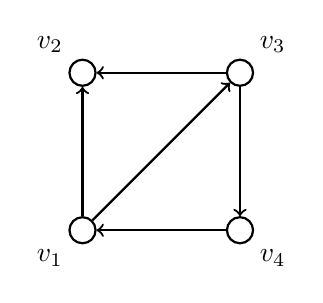
\begin{tikzpicture}[auto,
    specification/.style ={circle, draw, thick}]
   \node[specification] (A) [label=-135:$v_1$] at (0,0)  {};
   \node[specification] (B) [label=135:$v_2$] at (0,2)  {};
   \node[specification] (C) [label=45:$v_3$] at (2,2)  {};
   \node[specification] (D) [label=-45:$v_4$] at (2,0)  {};
   \draw[thick, ->] (A) to  (B);
   \draw[thick, ->] (C) to  (B);
   \draw[thick, ->] (C) to  (D);
   \draw[thick, ->] (D) to  (A);
   \draw[thick, ->] (A) to  (C);
 \end{tikzpicture}     
 \begin{Def}
   设$D=(V,A)$为一个有$p$个顶点$q$条弧的有向图,$V=\{v_1,v_2,\ldots, v_p\}$,$A=\{x_1,x_2,\ldots,x_q\}$,$p\times q$矩阵$H=(h_{ij})$称为$D$的关联矩阵,其中
  \[h_{ij}=\begin{cases}
      1, \text{如果}v_i\text{为弧}x_j\text{的起点}\\
      -1, \text{如果}v_i\text{为弧}x_j\text{的终点}\\
      0, \text{如果}v_i\text{既不是弧}x_j\text{的起点也不是弧}x_j\text{的终点}
    \end{cases}
  \]
 \end{Def}

   \begin{Def}
    一个有向图,如果抹去其所有弧的方向以后所得到的无向图是一棵无向树,则称该有向图为一棵{\bfseries 有向树}。
  \end{Def}

    \begin{Def}
    有向树$D$称为{\bfseries 有根树},如果$D$中恰有一个顶点的入度为0,而其余每个顶点的入度均为1。有根树中入度为0的顶点称为有根树的根,出度为0的顶点称为有根树的{\bfseries 叶子},非叶顶点称为有根树的{\bfseries 分支点}或{\bfseries 内顶点}。
  \end{Def}

    \begin{Def}
  设$T=(V,A)$为一棵有根树。如果$(u,v)\in A$,则称$v$为$u$的{\bfseries 儿子},$u$为$v$的{\bfseries 父亲}。如果从顶点$u$能达到顶点$v$,则称$v$为$u$的{\bfseries 子孙},$u$为$v$的{\bfseries 祖先}。如果$u$为$v$的祖先且$u \neq v$,则称$u$为$v$的{\bfseries 真祖先},$v$为$u$的{\bfseries 真子孙}。
  \end{Def}

    \begin{Def}
    设$T=(V,A)$为一棵以$v_0$为根的有根树。从$v_0$到顶点$v$的有向路的长度称为$T$的顶点$v$的{\bfseries 深度}。从顶点$v$到$T$的叶子的最长的有向路的长度称为顶点$v$在$T$中的{\bfseries 高度}。根顶点$v_0$的高度称为树$T$的{\bfseries 高度}。
  \end{Def}

    \begin{Def}
    设$T=(V,A)$为一棵有根树,$v$为$T$的一个顶点,由$v$及其子孙所导出的$T$的子图称为$T$的以$v$为根的{\bfseries 子树}。
  \end{Def}

    \begin{Def}
    设$T=(V,A)$为一棵有根树。如果$T$的每个顶点的各个儿子排定了次序,则称$T$为一
    棵{\bfseries 有序树}。
  \end{Def}

    \begin{Def}
    有序树$T$称为{\bfseries $m$元有序树},如果$T$的每个顶点的出度$\leq m$。一棵$m$元
    有序树$T$称为{\bfseries 正则$m$元有序树},如果$T$的每个顶点的出度不是$0$就是$m$。
    二元有序树简称{\bfseries 二元树}。
  \end{Def}




\chapter{}
%%% Local Variables:
%%% mode: latex
%%% TeX-master: "book_chapter10"
%%% End:
